\documentclass[10pt,twocolumn]{article}

\usepackage[T1]{fontenc}
\usepackage[utf8]{inputenc}
\usepackage[margin=0.70in,columnsep=0.24in]{geometry}
\usepackage{microtype}
\usepackage{graphicx}
\usepackage{booktabs}
\usepackage{tabularx}
\usepackage{array}
\usepackage{amsmath}
\usepackage{siunitx}
\usepackage{xcolor}
\usepackage[numbers,sort&compress]{natbib}
\usepackage[colorlinks=true,allcolors=blue!55!black]{hyperref}
\usepackage[font=small,labelfont=bf]{caption}
\usepackage{balance}

\newcommand{\code}[1]{\texttt{#1}}
\newcommand{\AUC}{\mathrm{AUROC}}
\newcommand{\dataset}[1]{\textit{#1}}
\renewcommand{\arraystretch}{1.08}
\setlength{\emergencystretch}{1.5em}
\hypersetup{
  pdftitle={When Dream Decoders Learn the Laboratory},
  pdfauthor={Javier Emilio Bazan Sanchez}
}

\title{When Dream Decoders Learn the Laboratory:\\
Cross-Dataset Validation and Reproducibility Audit of DREAM Experience Classification}
\author{Javier Emilio Baz\'an S\'anchez \quad
\normalsize\href{mailto:bazan@ciencias.unam.mx}{\texttt{bazan@ciencias.unam.mx}}}
\date{Draft prepared 2 August 2026}

\begin{document}
\maketitle

\begin{abstract}
Electroencephalographic classifiers that distinguish reports of dream
experience from reports of no experience appear to offer an objective window
onto otherwise private mental states. The DREAM database paper reported
above-chance discrimination in non-rapid-eye-movement (NREM) and rapid-eye-
movement (REM) sleep using pooled, randomly partitioned observations. We
audited the released Figure~5 workflow, reconstructed its public inputs, and
tested whether the reported signal transfers to unseen participants and unseen
laboratories. The code-path dataset comprised 1,065 strict binary reports from
five collections (730 NREM; 335 REM). A close adaptation recovered the
published scale of performance under record-wise splitting (NREM spectral
power, $\AUC=0.569$; REM band-filtered Catch22, $\AUC=0.636$), but performance
collapsed when an entire laboratory was held out ($0.493$ and $0.470$,
respectively). In contrast, source-dataset identity was strongly decodable
under participant-held-out validation ($\AUC=0.81$--$0.95$). Riemannian
covariance features and label-free log-Euclidean domain alignment did not
produce reliable transfer. Raw temporal-irreversibility features reached REM
$\AUC=0.604$ across laboratories, but fell to $0.490$ after normalization
against phase-randomized surrogates. Participant-cluster bootstrap intervals
did not exclude chance consistently in any target laboratory. The released
workflow also lacks a required feature module and expects a preformatted
Siclari representation absent from all public data versions inspected. These
results support within-pool discriminability but not a transportable EEG
marker of reported dream experience. Cross-laboratory validation and dataset-
identity controls should be treated as required falsification tests for
multicenter dream decoding.
\end{abstract}

\section{Introduction}

Dream reports create an unusual measurement problem: the target phenomenon is
a private experience, while the label becomes available only after awakening.
The DREAM database standardized multiple sleep EEG and mentation datasets to
enable larger-scale analyses of this problem \citep{wong2025dream}. In its
Figure~5 benchmark, XGBoost classifiers using normalized spectral power and
Catch22 time-series features discriminated ``Experience'' from ``No
experience'' in both NREM and REM sleep. The best reported mean areas under the
receiver-operating characteristic curve were $0.586$ for NREM spectral power
and $0.700$ for REM band-filtered Catch22.

These pooled results establish discriminability under the reported validation
scheme, but do not by themselves establish transportability. Multicenter EEG
datasets differ in hardware, reference, montage, filtering, awakening
protocol, class prevalence, and report semantics. A random split can therefore
place observations from the same participant and acquisition domain in both
training and test sets. Even when participants are separated, a model can use
stable laboratory signatures that remain shared across the split. This is a
general source of optimistic inference in machine-learning studies
\citep{varoquaux2018crossvalidation,kapoor2023leakage}.

We asked a stricter question: does a classifier trained on other DREAM
collections rank reported experience above no experience in a laboratory it
has never seen? We first audited the released code and public data. We then
implemented a validation ladder that changes only the train-test boundary:
random records, held-out participants, and a held-out laboratory. Finally, we
tested two mechanistically motivated extensions. Spatial covariance matrices
were analyzed on the symmetric-positive-definite manifold, an established EEG
transfer-learning framework \citep{barachant2012riemann,zanini2018transfer}.
Temporal irreversibility was tested because time-directed neural dynamics have
been proposed as a signature of conscious state \citep{delafuente2023time}.
Both extensions were paired with negative controls designed to expose domain
or spectral explanations.

\section{Materials and Methods}

\subsection{Source audit and inclusion}

We retrieved the versioned public DREAM collections named by the Figure~5 code
and verified every archive against its publisher-provided byte count and MD5
digest. We retained only strict binary labels: DREAM code 2 (Experience) was
mapped to 1 and code 0 (No experience) to 0. Experience without recall,
ambiguous labels, unknown labels, and wake observations were excluded. Four
official EDFs were unavailable for analysis: three files in the Young Adults
archive fail CRC despite the archive matching its published MD5, and one Turku
EDF is absent from its archive.

The paper describes six collections used across its broader EEG analyses. The
released Figure~5 classifier enumerates five. We separately audited the sixth,
Oudiette N1Data: its sleeping subset contains 23 strict Experience observations
and only one strict No-experience observation, and its Fp1/C3/O1 montage does
not match the classifier's F4/C4/O2 montage. It was therefore not inserted
post hoc into the classification analysis.

\begin{table*}[t]
\centering
\caption{Code-path datasets included in experience classification. Counts are
after label, stage, and file-integrity exclusions. Subject identifiers are
scoped to their source collection.}
\label{tab:data}
\begin{tabular}{lrrrrrr}
\toprule
Collection & Records & Subjects & No exp. & Experience & NREM & REM \\
\midrule
Zhang \& Wamsley 2019 & 212 & 28 & 56 & 156 & 186 & 26 \\
De Gennaro Multiple Awakenings & 435 & 19 & 121 & 314 & 281 & 154 \\
De Gennaro Young Adults & 62 & 62 & 24 & 38 & 32 & 30 \\
Tononi/Siclari Serial Awakenings & 231 & 39 & 107 & 124 & 231 & 0 \\
REM Turku & 125 & 18 & 3 & 122 & 0 & 125 \\
\midrule
Total & 1,065 & 166 & 311 & 754 & 730 & 335 \\
\bottomrule
\end{tabular}
\end{table*}

\subsection{Reproducibility gaps and explicit adaptations}

The deposited workflow could not execute literally against the current public
inputs for three reasons. First, it imports and calls \code{feat\_ext\_funcs},
which is absent from the code deposit. Second, it declares a semicolon delimiter
for De Gennaro Multiple Awakenings, while the public \code{Records.csv} is
comma-separated. Third, it searches for \code{formatted\_*.edf} files with
F4-M1, C4-M1, and O2-M1 channels for Siclari, whereas public versions 1--3
contain numerically named high-density channels and no formatted EDFs.

We made the minimum documented adaptations needed for a code-path
reproduction. Filtered Catch22 features were computed directly with
\code{pycatch22} \citep{lubba2019catch22}. Siclari F4/C4/O2-M1 signals were
reconstructed as HydroCel E224/E164/E150 minus E93, the nearest standard
HydroCel-256 sensors to F4/C4/O2/M1. Eight records without E93 used the nearest
available left-mastoid candidate. These choices make the analysis executable,
but prevent a claim of exact numerical reproduction.

\subsection{Signal processing and features}

We used the final 30~s preceding each report. Signals were resampled to 128~Hz
for time-series features. The replication families followed the released
workflow: (i) normalized multitaper power from 0.4--35~Hz, summed into delta
(0.5--4), theta (4.1--8), alpha (8.1--11), sigma (11.1--15), beta
(15.1--20), and gamma (20.1--35) bands across three channels (18 features);
(ii) 22 Catch22 features per broadband channel (66 features); and (iii) the
same features after each of six band-pass filters (396 features).

For geometric features, each broadband and band-limited epoch was represented
by a $3\times3$ covariance matrix $C$. We normalized $C$ by its trace, applied
one-percent identity shrinkage, and mapped it with the matrix logarithm. The
six unique tangent coordinates, with off-diagonal terms multiplied by
$\sqrt{2}$, were retained per band and broadband (42 features). A label-free,
transductive domain-alignment variant subtracted the log-Euclidean mean of each
laboratory and stage before classification.

Temporal irreversibility was summarized per channel at lags 1, 2, 4, and 8 by
(i) Jensen-Shannon divergence between forward and reversed ordinal-pattern
distributions of embedding dimension three and (ii) a signed cubic time-
asymmetry statistic. To separate nonlinear temporal ordering from spectral
effects, we generated 24 deterministic phase-randomized surrogates per channel
and expressed each statistic relative to its surrogate distribution.

\subsection{Classifier and validation ladder}

All binary models used the released XGBoost settings
\citep{chen2016xgboost}: learning rate 0.1, depth 3, subsampling 0.8, feature
subsampling 0.8, and the workflow's implicit default of ten boosting rounds.
No feature-family-specific hyperparameter search was performed.

Record-wise and participant-held-out results used five folds and 20 shuffled,
deterministic repetitions. Participant separation used stratified group
cross-validation. Laboratory-held-out analysis trained on all other
collections and evaluated the untouched collection once, separately for NREM
and REM. Because Siclari contributes only NREM and Turku only REM, each stage
has four eligible target laboratories. The primary cross-laboratory summary is
the unweighted mean of target-laboratory AUROCs. We also report a version in
which each target participant has equal metric weight. Uncertainty intervals
were obtained from 2,000 participant-cluster bootstrap samples within each
target laboratory.

As a negative control, we predicted dataset identity with the same features
using participant-held-out folds and macro one-versus-rest AUROC. High dataset
decodability indicates residual domain information but does not, on its own,
prove that every experience prediction is artifactual.

\section{Results}

\subsection{Random-split performance is approximately recoverable}

The adapted workflow recovered the scale and direction of the published
benchmark. NREM spectral power reached mean record-wise $\AUC=0.569$, compared
with $0.586$ reported in DREAM. REM band-filtered Catch22 reached $0.636$,
below the reported $0.700$, as expected given the absent feature module and
Siclari preprocessing. Holding out participants caused only modest changes and
did not expose the principal failure mode (Table~\ref{tab:ladder}).

\begin{table*}[t]
\centering
\caption{Validation ladder for reported-experience classification. Random-record
and new-subject values average five folds within each of 20 repetitions. New-
laboratory values are macro-averages across four target collections. The last
column gives the same laboratory-held-out ranking with equal total weight per
target participant.}
\label{tab:ladder}
\small
\begin{tabular}{llrrrr}
\toprule
Stage & Feature family & Random record & New subject & New laboratory & New lab., subject-equal \\
\midrule
NREM & PSD & 0.569 & 0.550 & 0.493 & 0.484 \\
NREM & Catch22 filtered & 0.574 & 0.555 & 0.441 & 0.444 \\
NREM & Riemannian covariance & 0.560 & 0.522 & 0.502 & 0.480 \\
NREM & Surrogate-normalized irreversibility & 0.554 & 0.548 & 0.520 & 0.512 \\
\midrule
REM & PSD & 0.596 & 0.593 & 0.481 & 0.497 \\
REM & Catch22 broadband & 0.639 & 0.616 & 0.573 & 0.561 \\
REM & Catch22 filtered & 0.636 & 0.663 & 0.470 & 0.455 \\
REM & Riemannian covariance & 0.642 & 0.640 & 0.544 & 0.523 \\
REM & Log-Euclidean alignment & 0.617 & 0.616 & 0.559 & 0.565 \\
REM & Temporal irreversibility & 0.599 & 0.612 & 0.604 & 0.589 \\
REM & Surrogate-normalized irreversibility & 0.608 & 0.628 & 0.490 & 0.464 \\
\bottomrule
\end{tabular}
\end{table*}

\begin{figure*}[t]
\centering
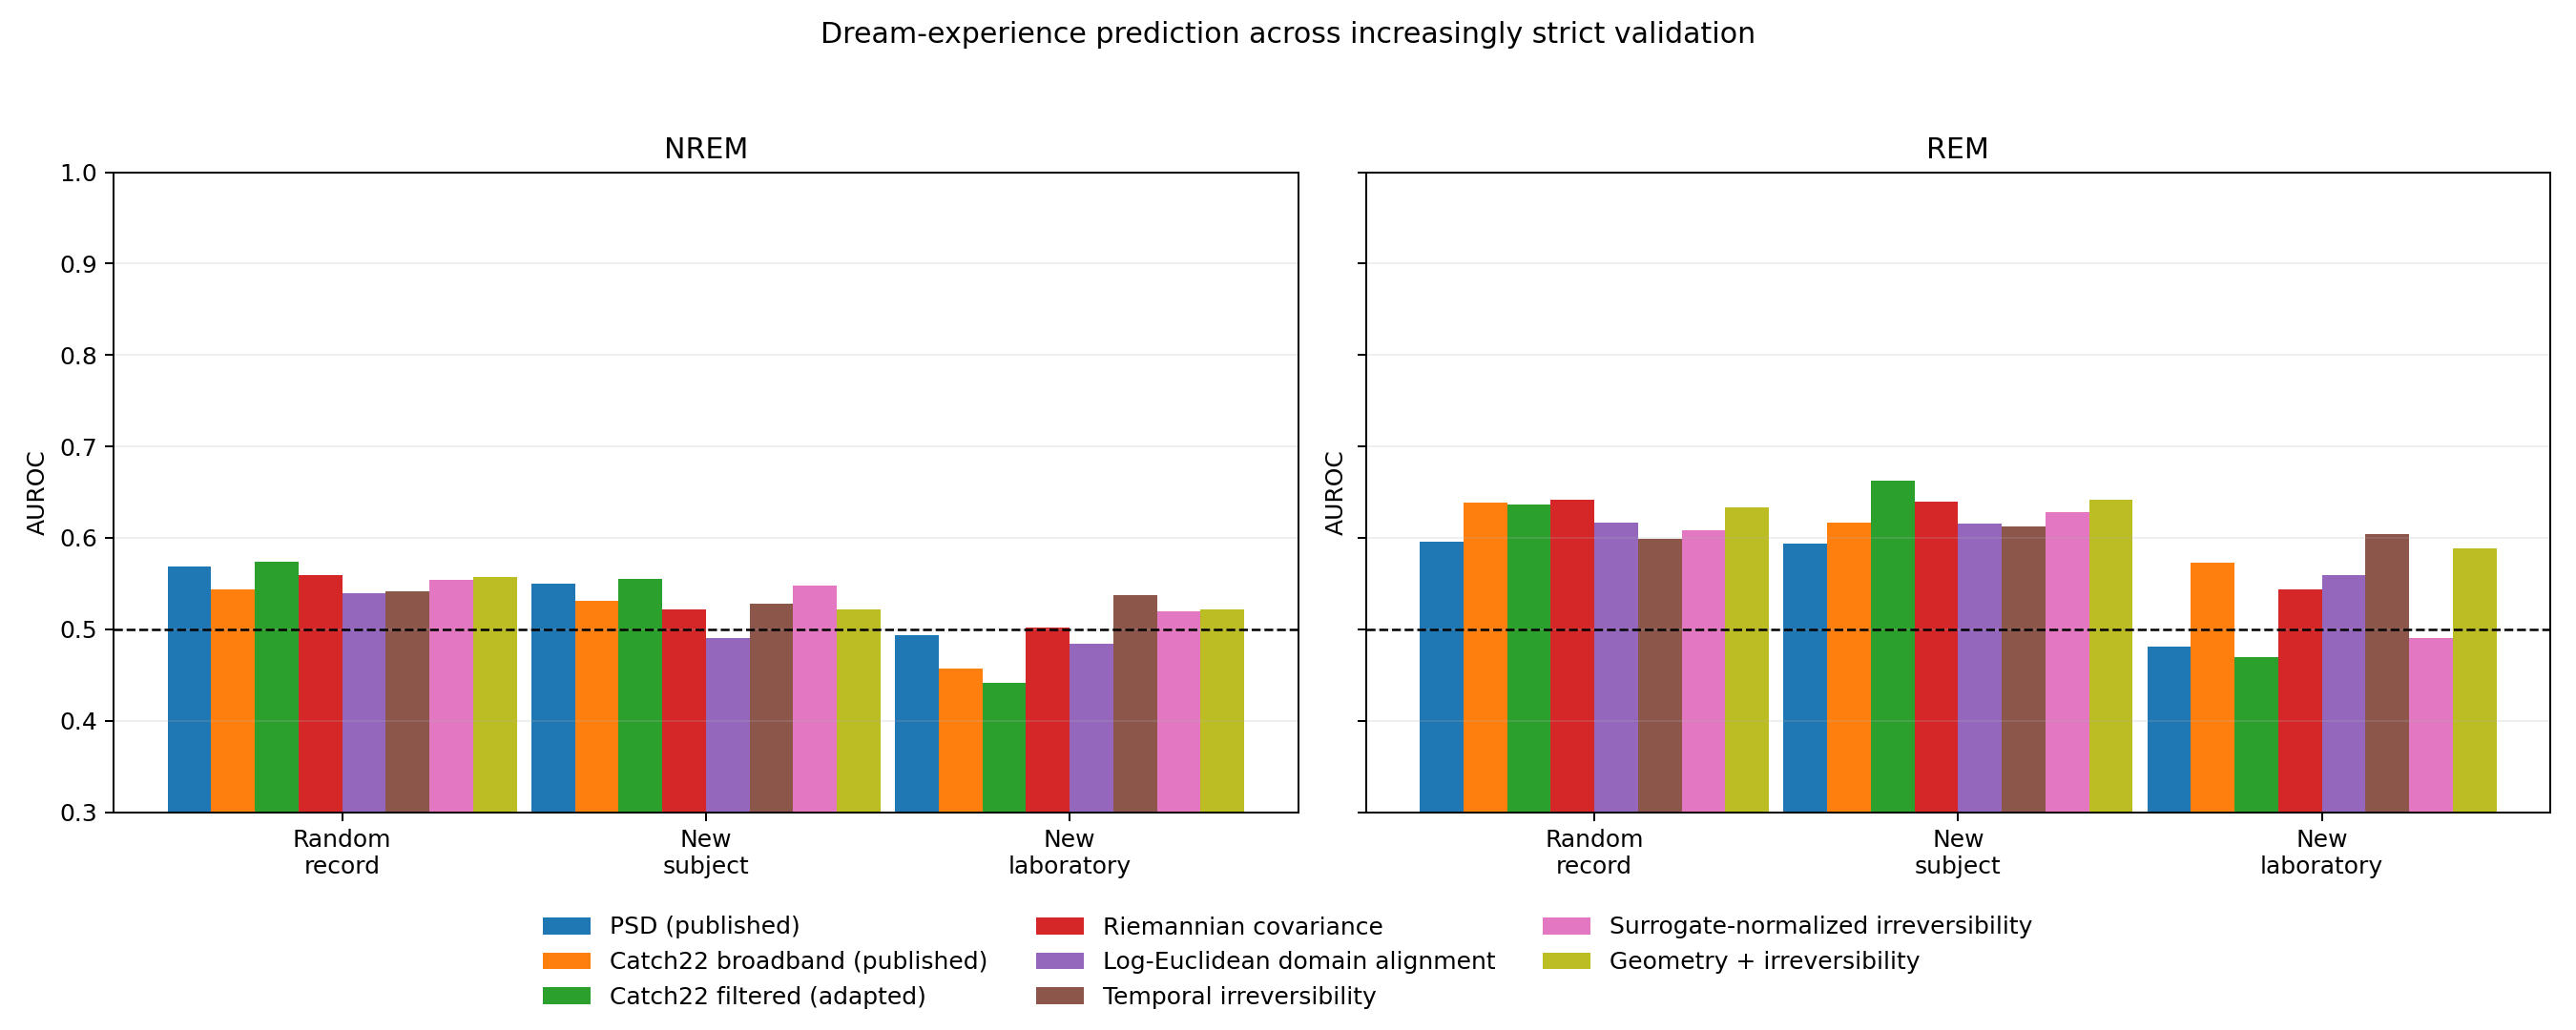
\includegraphics[width=0.98\textwidth]{figures/validation-ladder.png}
\caption{Experience-prediction AUROC across increasingly strict validation.
The dashed line marks chance ranking. Random-record and new-subject estimates
retain above-chance REM performance for several families; withholding a whole
laboratory produces large, method-dependent collapses. Bars show point
estimates and should not be interpreted as inferential intervals.}
\label{fig:ladder}
\end{figure*}

\subsection{Performance collapses under laboratory shift}

The published best-performing families did not transfer. NREM PSD fell from
$0.569$ under record splitting to $0.493$ across laboratories. REM filtered
Catch22 rose under participant separation ($0.663$) yet fell to $0.470$ when
the acquisition domain changed. Subject-equal estimates were $0.484$ and
$0.455$, respectively. At a probability threshold of 0.5, subject-weighted
balanced accuracy was approximately 0.5 for the REM cross-laboratory tests,
showing that calibration did not transport even when AUROC modestly exceeded
chance.

Target-specific uncertainty was substantial. No candidate produced a
favorable cluster-bootstrap interval excluding 0.5 in every target. REM
temporal irreversibility, for example, yielded subject-equal AUROC and 95\%
intervals of $0.725$ [0.500, 0.910] in Young Adults, $0.420$ [0.315, 0.536] in
Multiple Awakenings, $0.568$ [0.280, 0.860] in Zhang, and $0.642$ [0.363,
0.874] in Turku. The Turku estimate is especially fragile because only three
No-experience observations are available.

\subsection{Dataset identity dominates the feature space}

Dataset identity was strongly decodable despite participant-held-out
evaluation (Table~\ref{tab:identity}). Catch22 produced macro AUROC up to
$0.940$ in NREM and $0.953$ in REM. Riemannian covariance also retained strong
domain information. Log-Euclidean centering reduced NREM identity decoding
from $0.918$ to $0.770$, but did not reduce REM identity decoding materially
and improved REM experience transfer only from $0.544$ to $0.559$.

\begin{table}[t]
\centering
\caption{Participant-held-out dataset-identity AUROC.}
\label{tab:identity}
\begin{tabular}{lrr}
\toprule
Feature family & NREM & REM \\
\midrule
PSD & 0.839 & 0.808 \\
Catch22 broadband & 0.930 & 0.953 \\
Catch22 filtered & 0.940 & 0.912 \\
Riemannian covariance & 0.918 & 0.845 \\
Log-Euclidean alignment & 0.770 & 0.842 \\
\bottomrule
\end{tabular}
\end{table}

\subsection{Temporal asymmetry does not survive spectral control}

Unnormalized temporal-irreversibility features were the strongest exploratory
REM family under laboratory shift ($\AUC=0.604$ by record; $0.589$ with equal
participant weight). This advantage disappeared after normalization against
phase-randomized surrogates ($0.490$ and $0.464$). The surrogate procedure
preserves each channel's spectrum while disrupting nonlinear temporal order.
The reduction therefore argues against a domain-invariant arrow-of-time signal
in these features and favors spectral or acquisition-related explanations.

\section{Discussion}

This reanalysis distinguishes three claims that can otherwise be conflated.
First, DREAM EEG contains information that discriminates report labels under a
pooled random split; the approximate reproduction supports that claim. Second,
some of this information persists when participants are separated within the
same collection. Third, the resulting decision rule transports to a new
laboratory. The present evidence does not support the third claim.

The contrast between participant-held-out and laboratory-held-out performance
is particularly informative. REM filtered Catch22 improved after participant
separation yet inverted under domain shift. Thus, participant-level leakage is
not the only concern. Stable protocol and instrumentation signatures can remain
available on both sides of a participant-held-out split. The dataset-identity
control confirms that these signatures are large relative to the experience
signal.

Advanced mathematics did not automatically solve the domain problem.
Riemannian covariance is well motivated for multichannel EEG, but only three
common channels were available and their references were heterogeneous.
Label-free log-Euclidean centering removed a portion of the NREM site mean, not
the broader distributional differences. Likewise, temporal irreversibility had
an appealing theoretical connection to conscious dynamics, but the phase-
surrogate result showed why a targeted null model is essential before giving a
nonlinear feature a mechanistic interpretation.

The result should not be read as evidence that EEG contains no correlates of
dreaming. It shows that the tested representations and released workflow do
not yet establish a universal marker of a reported experience. Report labels
also remain imperfect proxies: ``No experience'' can combine absent
experience, failed encoding, forgetting, and protocol-specific categorization.
Cross-dataset failure may therefore reflect genuine construct heterogeneity as
well as measurement shift.

\subsection{Limitations}

This was an exploratory reanalysis rather than a prospective preregistration.
The missing feature module and unavailable preformatted Siclari files required
adaptations, and the filtered Catch22 result is not an exact reproduction.
Laboratory-held-out inference rests on four target domains per sleep stage,
with extreme REM imbalance in Turku. Only the common final 30~s and three
channels were analyzed. The domain-alignment analysis used the unlabeled target
batch and is therefore transductive. Our literature search did not locate an
earlier laboratory-held-out validation of this exact DREAM classifier, but it
was not a registered systematic review; novelty should be confirmed before
submission.

\section{Conclusion}

The DREAM Figure~5 signal is approximately reproducible under record-wise
validation but is not reliably transportable across laboratories. Dataset
identity is substantially easier to decode than reported dream experience,
and neither Riemannian alignment nor phase-controlled temporal
irreversibility provides a robust rescue. Multicenter dream-decoding studies
should report a validation ladder, dataset-identity negative controls,
participant-clustered uncertainty, and target-laboratory performance before
interpreting pooled accuracy as a general neural marker of private experience.

\section*{Data and code availability}

All source collections are public through the DREAM database and versioned
Figshare records. The analysis workspace records source URLs, file sizes, and
MD5 digests; scripts and fold-level outputs are frozen in local commit
\code{ebbaf97}. The \href{https://github.com/asim-v/dream-decoder-generalization-paper}{paper-only
public repository} contains the \LaTeX{} source, bibliography, figure, and PDF,
separate from raw and expanded EEG files. Exact numerical replication also
requires the unreleased
\code{feat\_ext\_funcs} implementation and the preformatted Siclari files
expected by the deposited workflow.

\section*{Ethics statement}

This study reanalyzed de-identified, publicly released data and did not recruit
participants or modify source records. Ethical approvals and consent procedures
are described in the originating studies and DREAM data records.

\section*{Competing interests}

The author declares no competing interests.

\balance
\bibliographystyle{unsrtnat}
\bibliography{references}

\end{document}
